\section{Data}

% \cite{2015AnA...578A.114F} HIPS

\begin{enumerate}
\item Survey images

  \begin{itemize}

  \item Default: Fermi color image. Mention other survey options

  \item HiPS file format and HEALPix projection for the map

  \item Our images came from CDS' HiPS database of 300+ images

  \end{itemize}


\item Catalog images

  \begin{itemize}

  \item Fermi-LAT - 3FGL and 2FHL

  \item SNRcat

  \item GeTeV Catalogue

  \end{itemize}
\end{enumerate}


\begin{figure}[tb]
  \centerline{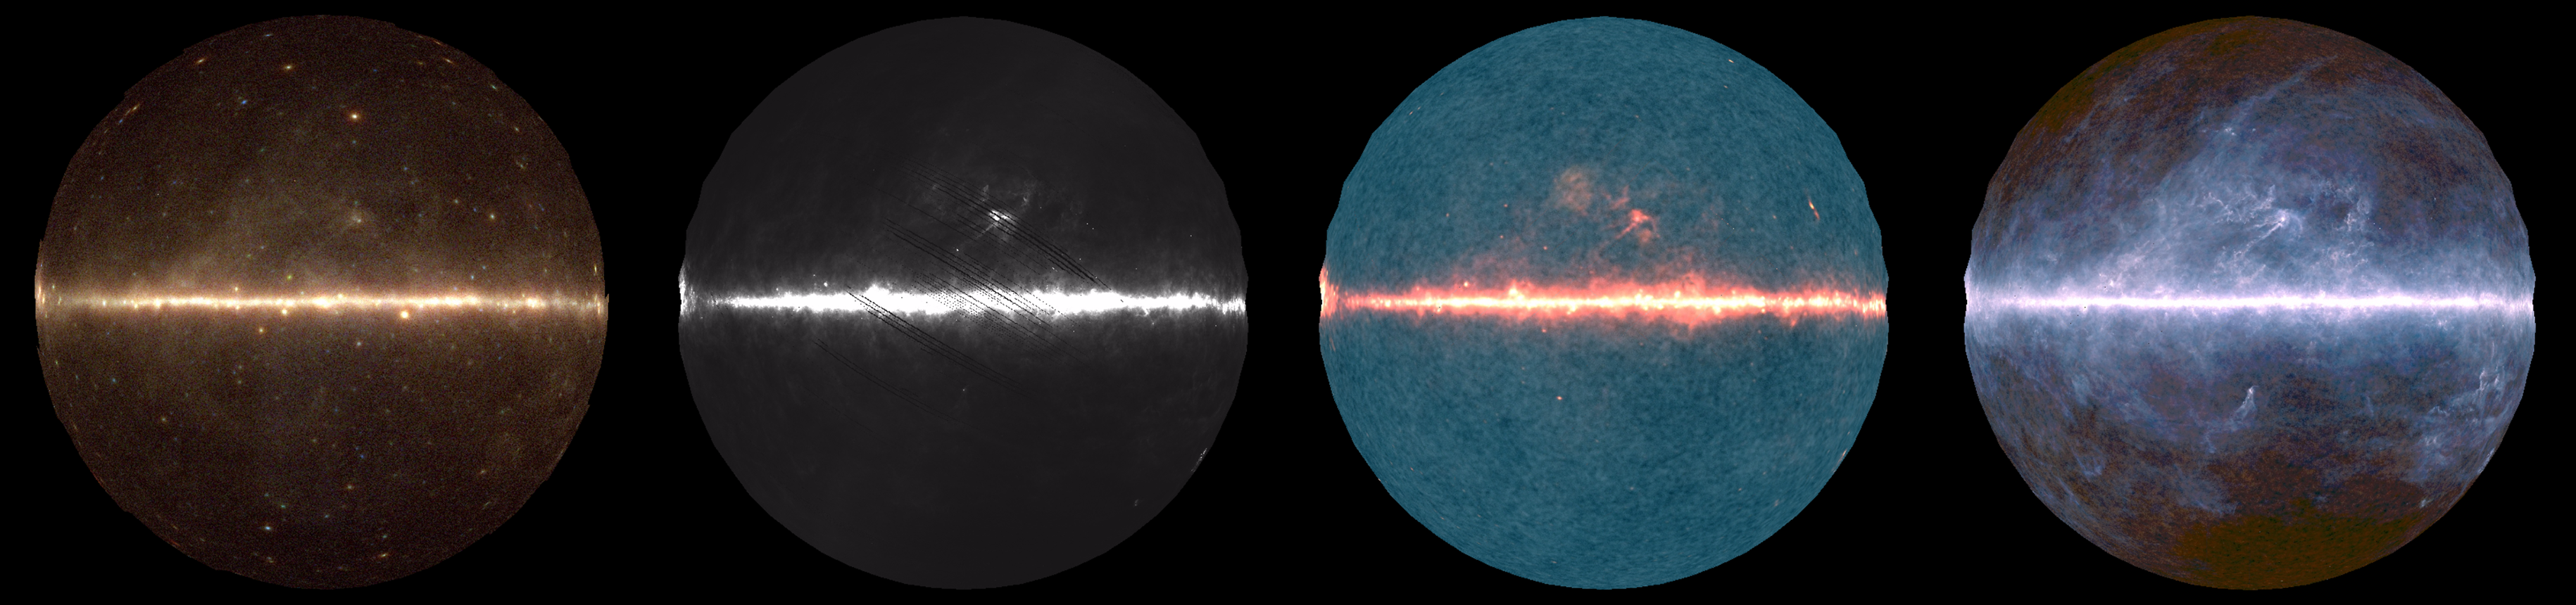
\includegraphics[width=\textwidth]{figures/four_images}}
  \caption{Survey images (left to right): Fermi color, AKARI 90um, Planck LFI, Planck HFI.
           Images centered on the Galactic Center, FOV 180 degrees.}
\end{figure}

\begin{figure}[tb]
  \centerline{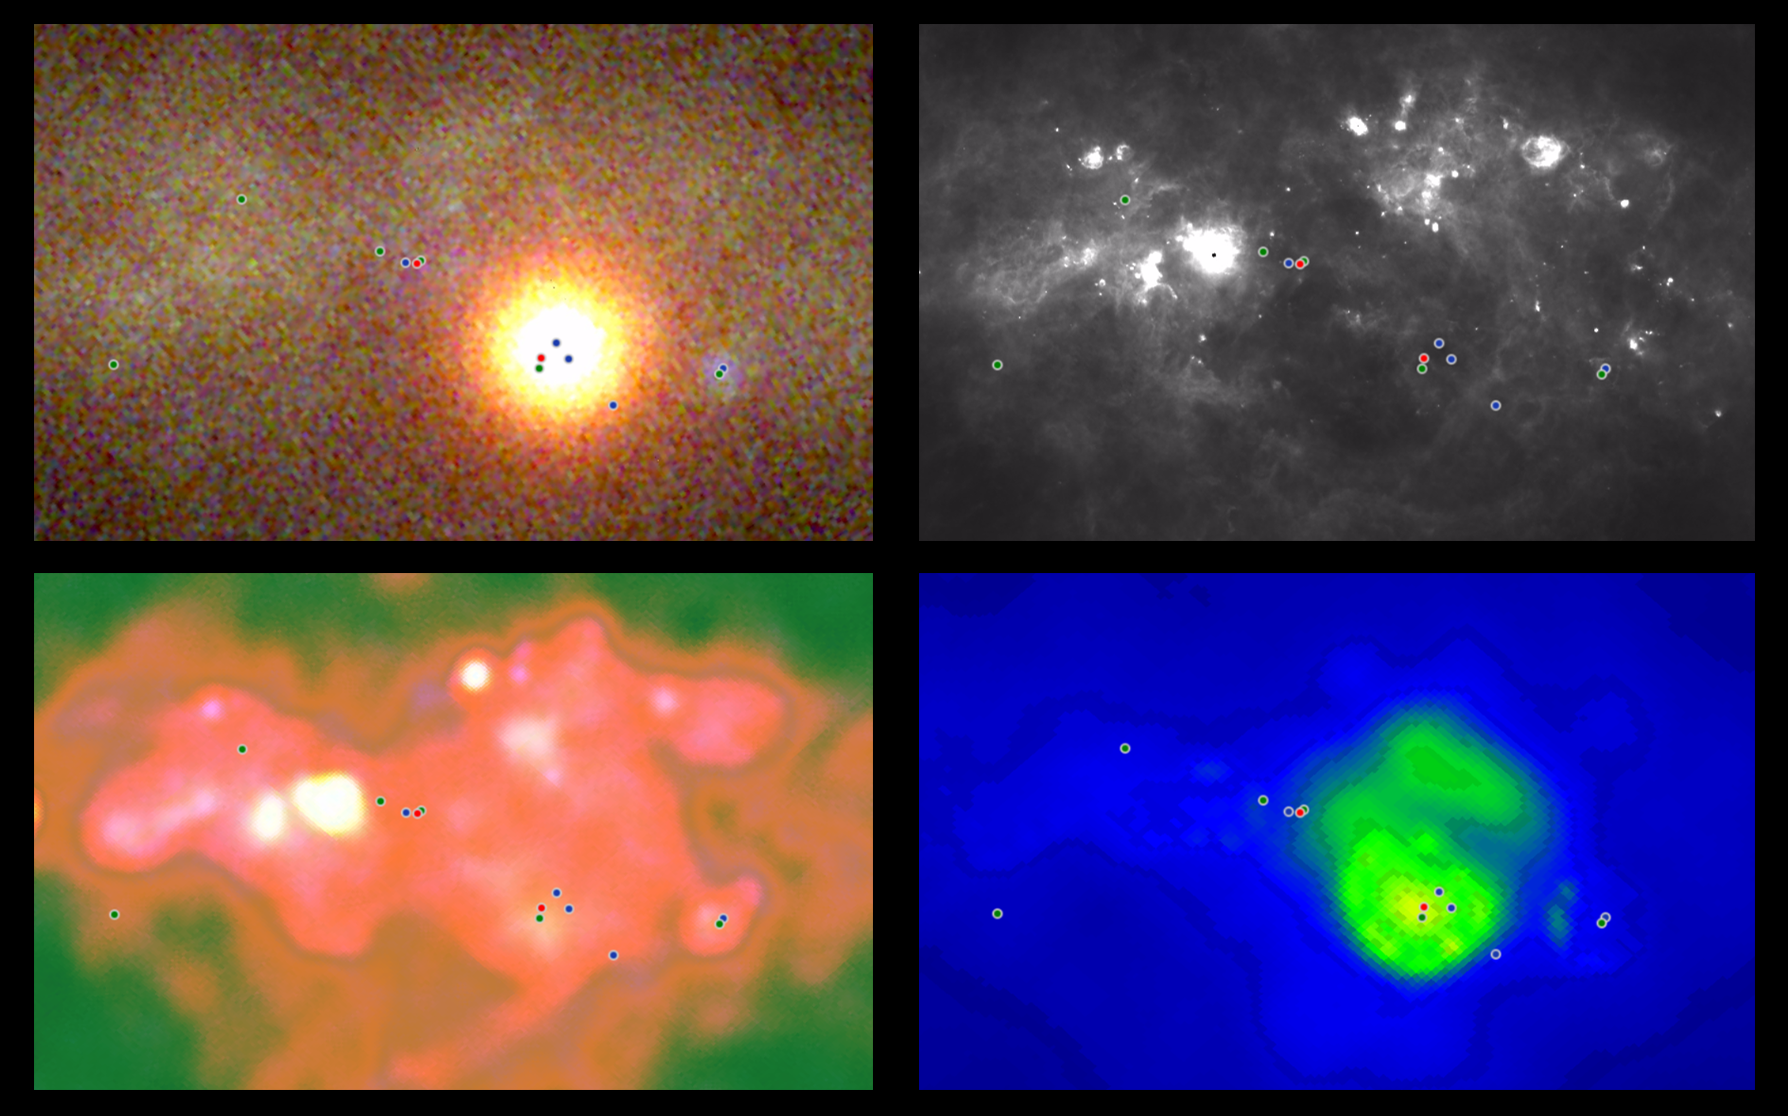
\includegraphics[width=\textwidth]{figures/vela_region}}
  \caption{The Vela Region in various survey images and color maps, FOV 20 degrees.}
\end{figure}

% \begin{figure}[tb]
%   \centerline{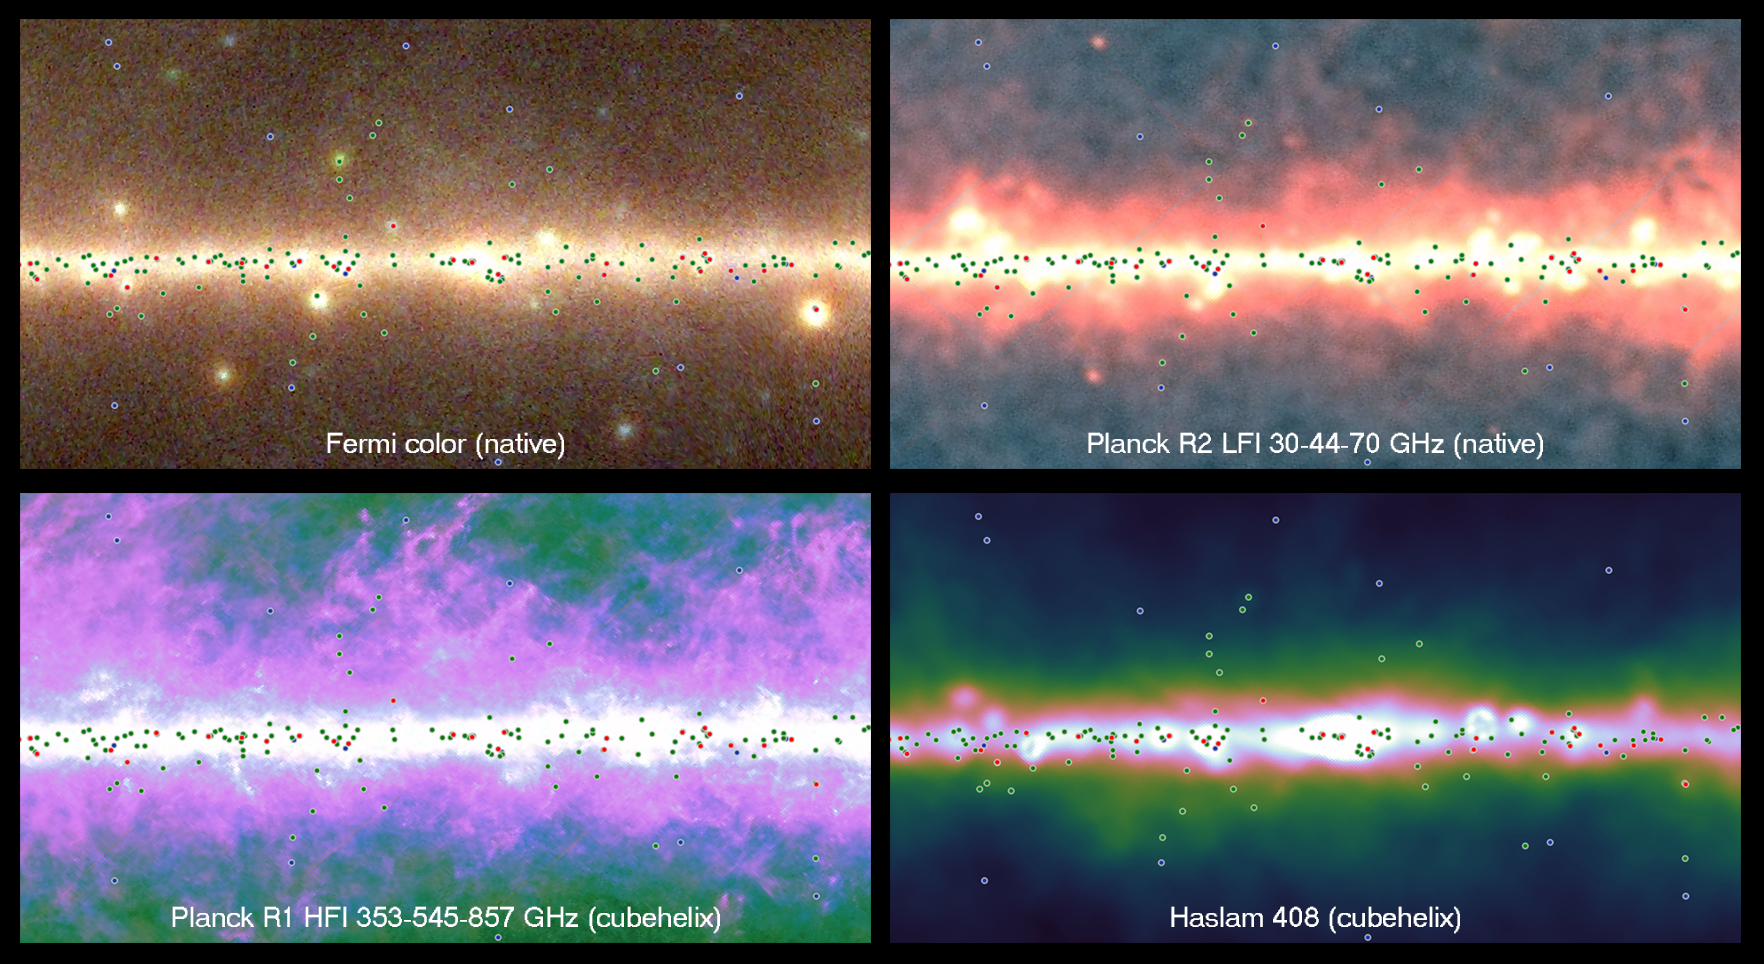
\includegraphics[width=\textwidth]{figures/inner_galaxy_region}}
%   \caption{The inner Galaxy in various survey images and color maps, FOV 45 degrees.}
% \end{figure}

% \begin{figure}[tb]
%   \centerline{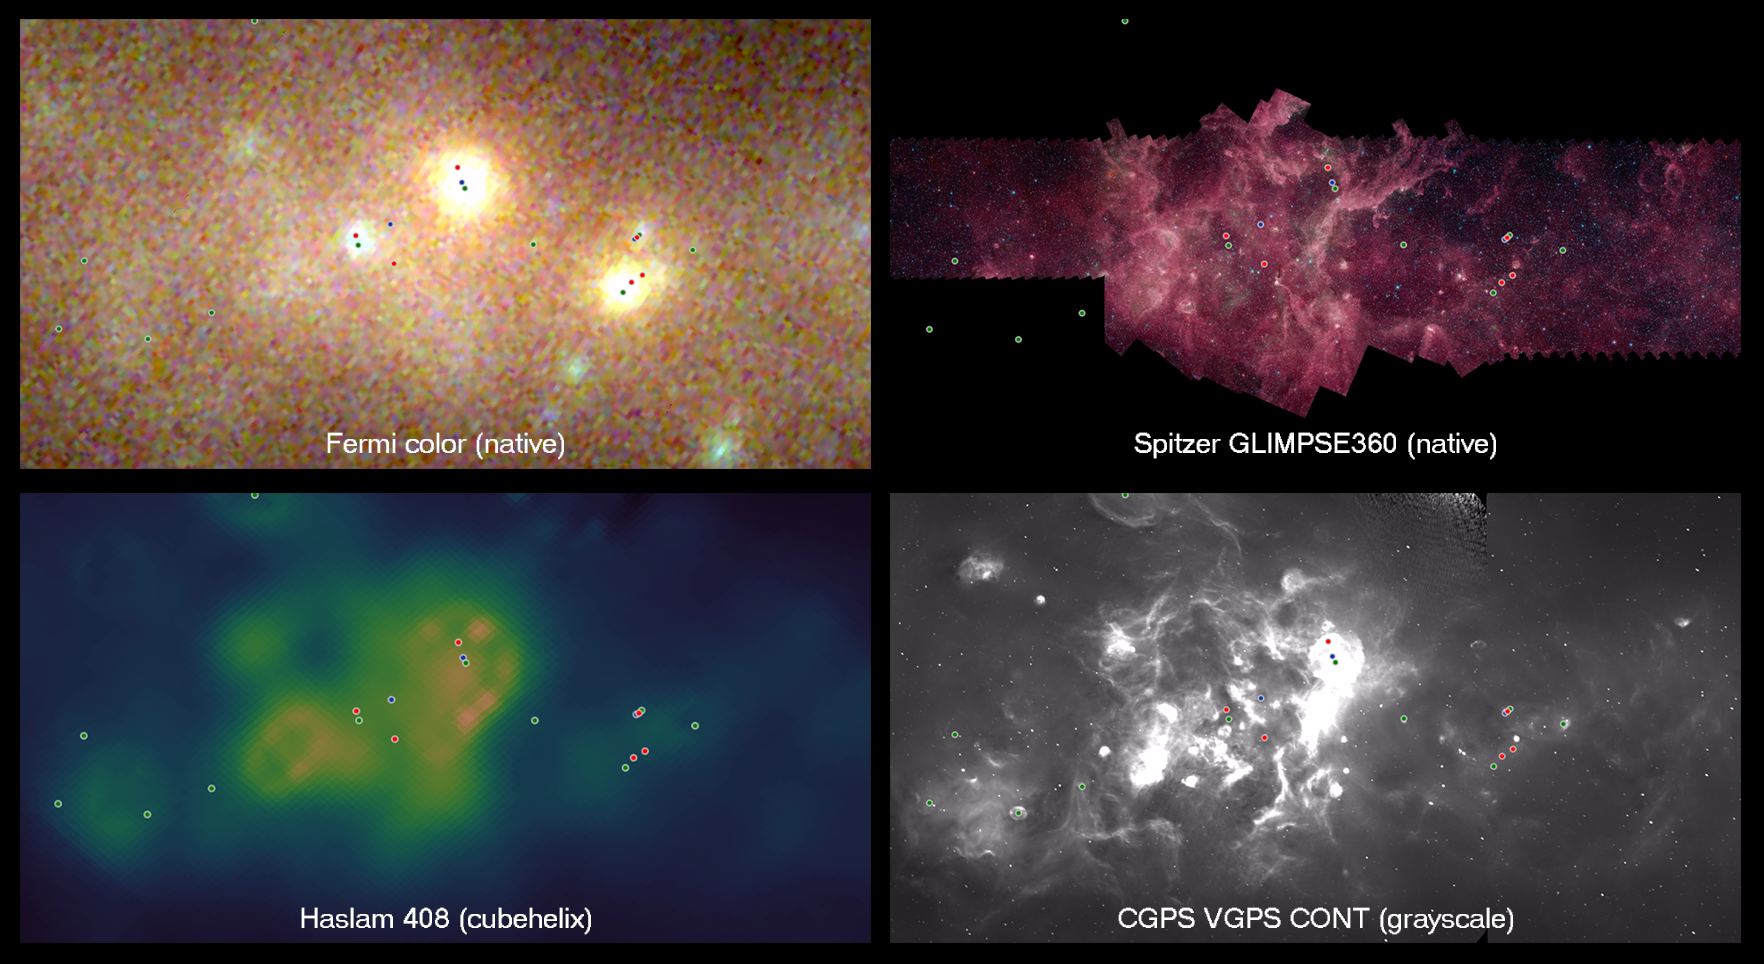
\includegraphics[width=\textwidth]{figures/cygnus_region}}
%   \caption{The Cygnus Region in various survey images and color maps, FOV 20 degrees.}
% \end{figure}

\begin{figure}[tb]
  \centerline{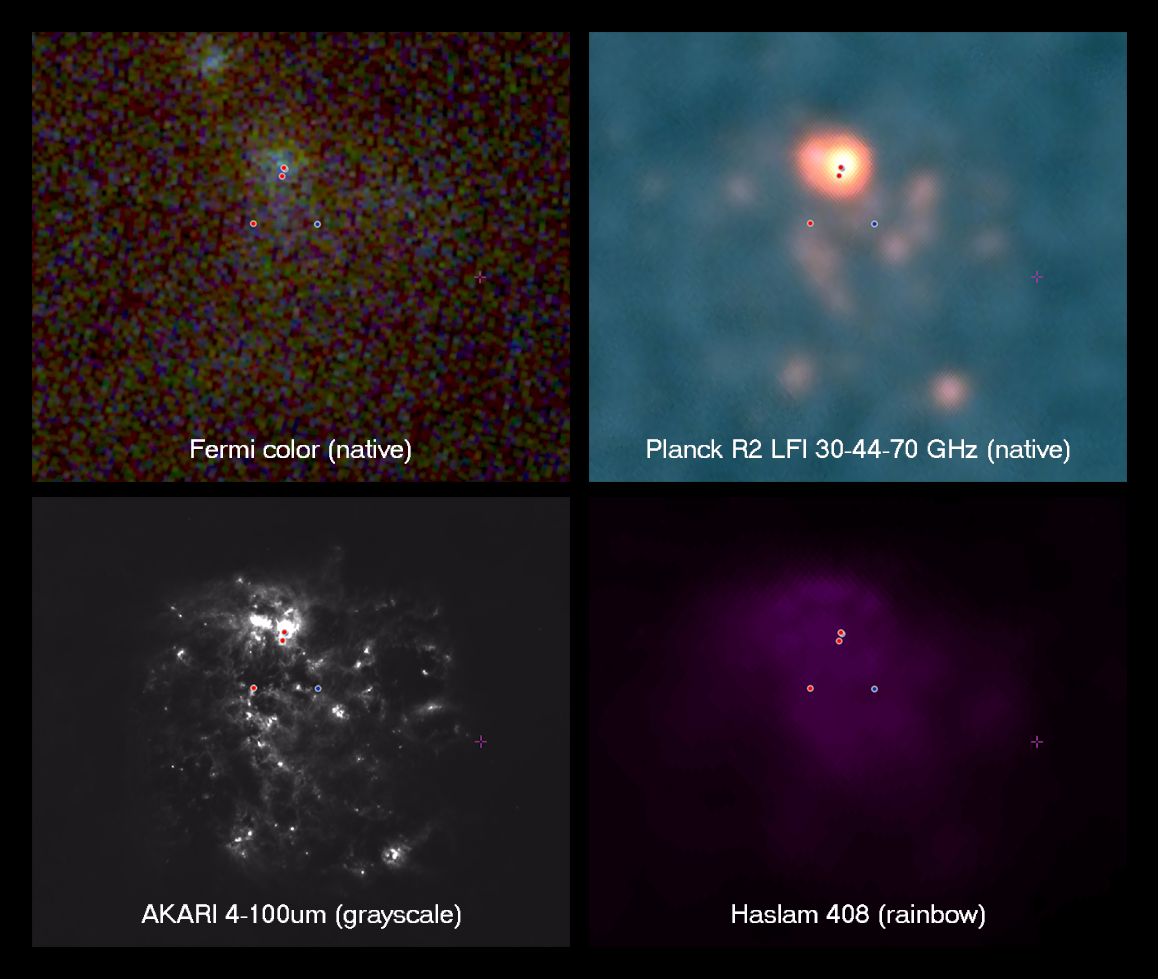
\includegraphics[width=\textwidth]{figures/LMC_region}}
  \caption{The Large Magellanic Cloud in various survey images and color maps, FOV 10 degrees.}
\end{figure}



\begin{table}[bt]

\caption{
Source catalogs currently displayed on \gammasky .
We intend to add additional catalogs of interest to gamma-ray astronomers to the website in the future, including the upcoming H.E.S.S. and HAWC TeV source catalogs, as well as the ATNF Pulsar Catalogue.
}
\label{tab:catalogs}
\tabcolsep7pt\begin{tabular}{ lrll }
\hline
Catalog   & Sources & Updates    & Description \\
\hline
gamma-cat &     153 & continuous & Open TeV gamma-ray source catalog  \\
&&& \gammacat  \\
2FHL      &     360 & fixed      & Second Fermi-LAT catalog of high-energy sources \citep{2fhl}\\
&&& \url{http://fermi.gsfc.nasa.gov/ssc/data/access/lat/2FHL/}  \\
3FGL      &    3034 & fixed      & Third Fermi-LAT point source catalog \citep{3fgl}\\
&&& \url{http://fermi.gsfc.nasa.gov/ssc/data/access/lat/4yr_catalog/}  \\
SNRcat    &     378 & continuous & A census of high-energy observations of Galactic supernova remnants \citep{snrcat}\\
&&& \url{http://www.physics.umanitoba.ca/snr/SNRcat/} \\
\hline
\end{tabular}
\end{table}


\begin{table}[bt]

\caption{
Survey images of interest to gamma-ray astronomers available on \gammasky . Note that this is only a very small selection, there are over 300 other multi-wavelength survey images available from CDS via Aladin Lite. The ones listed here were not produced by us specifically for \gammasky . We plan to add more gamma-ray survey images from the GeV energy range (high-energy Fermi-LAT data) and the TeV energy range (H.E.S.S. Galactic plane survey).
}
\label{tab:images}
\tabcolsep7pt\begin{tabular}{ lrlrl }
\hline
Image & Resolution (arcmin) & Type & Band & Coverage\\
\hline
Fermi-LAT & TBD & gamma-ray &  & all-sky\\
AKARI 90um & 1 & infrared &  & all-sky\\
CGPS-VGPS CONT & 1 & radio &  & galactic plane\\
Haslam 408 & 51 & radio & 408 MHz & all-sky\\
IRIS Band 4-100um & TBD & infrared &  & all-sky\\
Planck R1 + R2 HFI & TBD & microwave & 353-545-857 GHz & all-sky\\
Planck R2 LFI & TBD & microwave & 30-44-70 GHz & all-sky\\
Spitzer GLIMPSE360 & 0.02 & infrared &  & galactic plane\\
\multicolumn{5}{c}{300+ other HIPS survey images available from \url{http://aladin.u-strasbg.fr/hips/list}} \\
\hline
\end{tabular}

\end{table}

